\section{Design}
\begin{figure*}
    \centering
    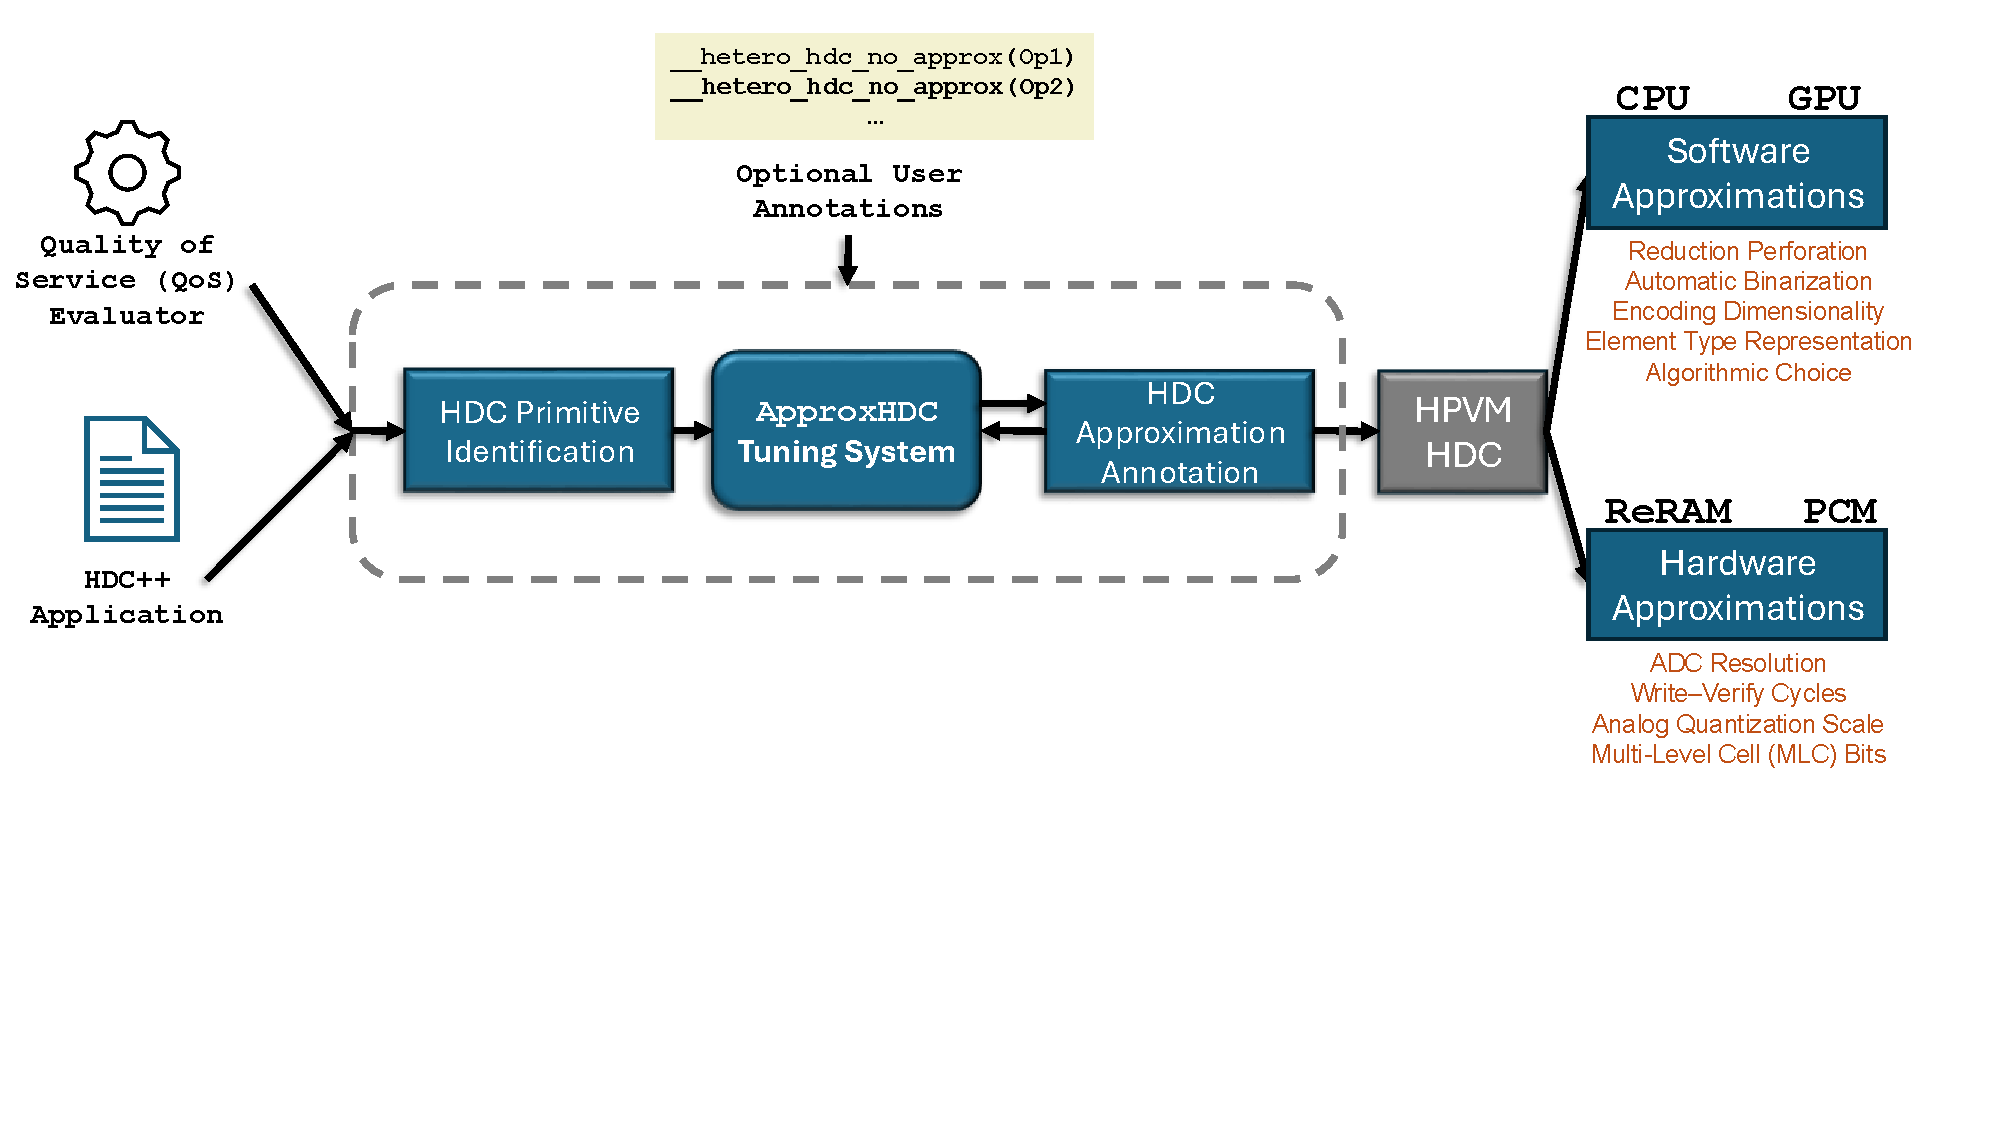
\includegraphics[width=0.75\linewidth]{figures/ApproxHDC Workflow.pdf}
    \caption{Overview of the \pname{} workflow. Given HDC applications written in HDC++ along with an application-specific quality-of-service (QoS) evaluator, \pname{} first extracts the set of HDC primitives used in the program. It then performs efficient autotuning to explore approximation choices at both the global and per-operation levels. Finally, \pname{} applies the selected approximations via automatically generated source-level annotations, ensuring that the specified QoS constraints are satisfied. The search space considered by \pname{} spans both software- and hardware-level approximations.}
    \label{fig:overall-workflow}
\end{figure*}
\label{sec:design}
\pname{} is implemented as an extension to the HPVM-HDC compiler through two dedicated compiler passes. Leveraging the approximation specification mechanism provided by HDC++, where approximation types and their parameters can be expressed via in-program source annotations (Section~\ref{bg:hdc++}), \pname{} automatically selects and applies appropriate approximations. Specifically, \pname{} encodes its decisions by inserting the corresponding annotations directly into the HDC++ application, enabling seamless integration with the existing compilation and optimization pipeline. This enables \pname{} to exist externally to the compiler and be easily modified without needing to recompile the HPVM-HDC compiler (which is written in C++). The overall compilation flow is shown in Figure~\ref{fig:overall-workflow}.

\textbf{HDC Primitive Identification.}
The first compiler pass performs a static analysis of the HDC++ application code (prior to the introduction of any approximations) to identify all invocations of HDC primitives used in the program. Each primitive instance is uniquely characterized by its context, which includes the enclosing function and basic block. When multiple occurrences of the same primitive appear within a single basic block, they are further disambiguated based on their execution order within that block. The identified primitives, along with their contextual metadata, are aggregated into a serializable JSON representation, enabling external tools such as \pname{} to access a structured view of the program’s HDC operations (see Listing~\ref{lst:approx_interface}).

\lstinputlisting[caption={Interface for \pname{} emitted from HPVM-HDC for approximation tuning.}, label={lst:approx_interface}]{code_snippets/primitive_desc_for_tuner1}


\textbf{ApproxHDC Tuning System.}
After identifying the HDC primitives within the application, the \pname{} Tuning System constructs the approximation design space to be explored. This space encompasses both software-level approximations, which are applicable across general-purpose hardware targets such as CPUs and GPUs, and hardware-specific approximations, which target specialized architectures including HD-PCM and HD-ReRAM. The specific types of approximations supported are detailed in Section~\ref{sec:approx-tuning-system}.
To evaluate the impact of different approximation choices, the user provides an application-specific driver that executes the program with the appropriate command-line arguments and datasets, and reports a quality-of-service (QoS) metric (e.g., inference accuracy). The \pname{} Tuning System then empirically explores multiple approximation configurations, measuring QoS, execution time, and energy consumption. \pname{} can be tuned for either end-to-end performance or energy efficiency, subject to a specified QoS constraint.
For each evaluated configuration, the system generates a JSON representation (consistent with the format produced by the HDC Primitive Identification pass) that records the selected approximations and their parameterizations (see Listing~\ref{lst:approx_interface_from_tuner}). Each operation may be assigned zero, one, or multiple approximations. The tuning system further supports user-defined approximation parameters, enabling extensibility to new approximation techniques and hardware targets. By default, the tuning system constructs the approximation space across all HDC operations present in the application. Section~\ref{sec:approx-tuning-system} describes the mechanisms provided by \pname{} to customize and constrain this space, allowing fine-grained control over which operations and approximation parameters are explored.

\lstinputlisting[caption={Interface emitted from the \pname{} Tuning System to specify fine-grained, per-operation approximation configurations.}, label={lst:approx_interface_from_tuner}]{code_snippets/approx_hdc_tuning_config}
%\vspace{-0.40cm}

\textbf{HDC Approximation Application.}
The second compiler pass consumes the fine-grained approximation configurations produced by the tuning system (as illustrated in Listing~\ref{lst:approx_interface_from_tuner}) and automatically inserts the corresponding source-level approximation annotations into the HDC++ application. Leveraging the contextual metadata collected during the primitive identification phase, each instance of an HDC primitive can be uniquely identified and independently annotated, enabling the application of distinct approximation strategies to different occurrences of the same primitive.

\textbf{Compilation and Execution.}
The HPVM-HDC compiler is employed to perform the necessary compiler transformations specified by the inserted source-level annotations. Section~\ref{sec:approx-tuning-system} describes the set of supported software and hardware approximations, including those developed as part of \pname{}. Using the user-provided application driver, the annotated HDC++ program is compiled and executed, and the corresponding quality-of-service (QoS) metric is recorded. These results are then fed back to the \pname{} Tuning System, which uses them to guide the selection of subsequent approximation configurations. The tuning process continues iteratively until a specified time budget or iteration limit is reached, at which point it outputs the final approximation configuration that maximizes the chosen objective function.
%\vspace{-0.75cm}